\EnglishSourceFrame{GELFAND-P001435}{10}
\EnglishUnclear{GELFAND-P001435}{heading-date}{22.2.88 / 22.2.82}
\underline{Angles between subspaces.}

\begin{center}
\underline{A series of problems about angles between subspaces}

(\underline{I.M. Gelfand}; from A.K. Zvonkin's notes)
\end{center}

Some are accessible to an eighth-grade pupil (problems in $R^2$ and $R^3$),
others are for a Doctor of Sciences (problems in Hilbert space).

What is the ``angle'' between two lines in the plane?
It is an orthogonal invariant of this pair of lines, i.e. a numerical
characteristic that does not change under any orthogonal transformation
of the plane.

Moreover, the angle is a \underline{complete system of invariants}, i.e.
one pair of lines can be carried into another pair by an orthogonal transformation
if and only if these two pairs of lines have the same angle.

In what follows, ``angle'' means a complete system of
invariants of an object under the action of a group.
Sometimes it is a number, sometimes a finite or countable set of numbers,
and sometimes even a continuum of numbers.

(When discussing, say, a quadruple of subspaces of
$\Rightarrow$ [arrow continuing the line]
a linear space, we shall not use the expression ``\underline{angle between\ldots}'',
since it is unclear between what; instead we shall say ``\underline{angle for\ldots}''.)

In all the problems, it is of interest not only to determine
\underline{what an angle is}, but also \underline{what values it can
take}.

\paragraph*{I. \underline{Problems for school pupils.}}
1. What is the angle between a line and a plane in three-dimensional
space?

(Two versions: the line is oriented or unoriented.)

2. What is the angle between two planes in three-dimensional
space?

\paragraph*{II. \underline{Problems for university students.}}
3. A 4-dimensional linear space with an inner product is given.
(Not $R^4$, since no axes are distinguished.) What is the angle between two of its
two-dimensional subspaces?

4. Given $\{L,(\cdot,\cdot)\}$, $\dim L=n$, $v\in L$, $V\subset L$,
$\dim V=k$.

Determine the angle between $v$ and $V$.

\EnglishSourceFrame{GELFAND-P001436}{unlabelled}
5. Given $\{L,(\cdot,\cdot)\}$, $\dim L=n$, $V,W\subset L$,
$\dim V=k$, $\dim W=m$. Determine the angle between $V$ and $W$.

6. Let $L$ be simply a linear space (without an inner
product). Determine the angle for

(a) a subspace of $L$

(b) a pair of subspaces

(c) a triple of subspaces.

(The group here is to be understood as $GL(n)$.)

7. A Minkowski plane is given, i.e. $L$, $\dim L=2$
with the indefinite inner product $-x_1^2+x_2^2$.
Determine the angle between two lines (i.e. an invariant
under the group of transformations preserving this
inner product).

8. Further variations:
\begin{itemize}
\item[---] for a higher-dimensional Minkowski space
and two of its subspaces
\item[---] for other spaces with an indefinite metric
(i.e. with more than one minus sign in the inner product)
\item[---] for spaces with a degenerate form (for example, $R^3$
with the inner product $x_1^2+x_2^2$).
\end{itemize}

For all the listed problems, consider the cases of the
groups $O(n)$ and $SO(n)$.

\paragraph*{III. \underline{Problems for postgraduate students.}}
9. A linear space $L$ and a quadruple of its subspaces are given. Find the angle
for this quadruple (this is the content of Gelfand and Ponomarev's work).

10. (A.A. Kirillov, Jr.) Given $\{L,(\cdot,\cdot)\}$; an inner
product is then also defined on the tensor powers of $L$. Let
$a,b\in L\otimes L$. Find the angle between the subspaces $a\otimes L$ and
$L\otimes b$, embedded in $L\otimes L\otimes L$.

(This is needed for Hecke algebras and the Yang--Baxter equation.)

\EnglishSourceFrame{GELFAND-P001437}{11}
\paragraph*{IV. \underline{Problems for Candidates and Doctors of Sciences.}}
11. Determine the angle for two subspaces of a Hilbert space.
Give examples in which the value of the angle is a countable
set of numbers, and ones in which it is a continuum of numbers.

12. The same problem for a Hilbert space with an indefinite metric.

\paragraph*{\underline{Comments.}}
1. In these problems, the second part is especially difficult; for example,
given a subspace and an angle, construct
another subspace making the given angle with the given one.

2. A linear operator can be specified by means of
a quadruple of subspaces.

\EnglishSourceFrame{GELFAND-P001438}{unlabelled}
\underline{21/III-88} \qquad \underline{Gelfand's seminar}

\underline{\underline{A. Radul.}}

\paragraph*{\underline{Quantum Gelfand--Dickey brackets}}
(following S. Lukyanov) \qquad Consider on $S^1$ the operator
\begin{equation*}
L=\partial_z^N+\sum_{i=0}^{N-1}u_{N-1}(z)\partial_z^i . \tag{1}
\end{equation*}
\EnglishUnclear{GELFAND-P001438}{operator-coefficient}{Coefficient index: $N-1$ / $N-i$.}

and the space of functionals of the form
\begin{equation*}
f[u]=\oint P\bigl[z,u_i^{(k)}(z)\bigr]dz \tag{2}
\end{equation*}
and their finite products; $P$ is a polynomial in $u_i^{(k)}$.

Two Gelfand--Dickey brackets are defined on such functionals
\begin{equation*}
\frac{\delta f}{\delta u_i}\quad
\text{defined by the relation:}\quad
\left.\frac{d}{d\varepsilon}f[u+\varepsilon\delta u]\right|_{\varepsilon=0}
=\oint dz\,\frac{\delta f}{\delta u_i}\delta u_i . \tag{3}
\end{equation*}

\underline{I.M. Gelfand}
\paragraph*{\underline{Digression on functional analysis}}
All the intuition of functional analysis came from the idea that functionals are also
functions, but on an $\infty$-dimensional space.

I.M.G. changed his point of view, with two consequences.

1) Functionals can be of different types, and must be classified.

2) Functionals are not functions $\Rightarrow$ this affects geometry.

1) In the calculus of variations, there are functionals
\begin{equation*}
\int_0^L f\bigl(x,u(x),u'(x)\bigr)\,dx \tag{*}
\end{equation*}
\EnglishUnclear{GELFAND-P001438}{local-functional-argument}{Argument of the middle $u$: $x$ / $z$.}

This is a functional of $u$, but it has the property:

\EnglishSourceFigure{GELFAND-P001438}{locality-diagram}{A sloping line with two upward protrusions; no labels or arrows are visible. There are breaks in the strokes at the tops of the protrusions.}

\par\medskip\noindent
\begin{minipage}[c]{0.48\linewidth}\centering
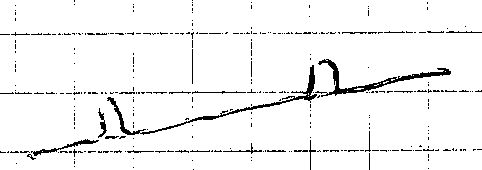
\includegraphics[width=\linewidth]{figures/gelfand-p001438-locality-diagram-original.png}
\par\smallskip{\footnotesize Original manuscript diagram: GELFAND-P001438\par}
\end{minipage}\hfill
\begin{minipage}[c]{0.48\linewidth}\centering
\resizebox{\linewidth}{!}{% Partial trace of the visible source strokes, in original crop-pixel coordinates.
% No coordinate axes, function values, arrowheads or missing joins are inferred.
\begin{tikzpicture}[x=0.01cm,y=-0.01cm,line width=0.55pt]
\path[use as bounding box] (0,0) rectangle (482,170);
\draw (29,155)--(55,147)--(81,140)--(94,141);
\draw (99,138)--(105,131)--(99,113);
\draw (108,99)--(117,112)--(121,131)--(132,137)
 --(154,132)--(185,121)--(223,113)--(253,108)--(281,102)--(309,96);
\draw (309,96)--(313,87)--(313,66);
\draw (321,62)--(329,61)--(334,68)--(335,88)--(338,94)
 --(356,93)--(380,86)--(404,79)--(426,75)--(446,73);
\draw (441,69)--(449,70)--(451,73);
\end{tikzpicture}
}
\par\smallskip{\footnotesize Partial recreation of visible strokes; gaps remain unjoined.\par}
\end{minipage}\par\medskip


if there is an increment [inserted above the line, with an arrow to this point: $u$]
at two places, then
the increment of the functional (*) will be the sum of
[crossed out: \EnglishUnclear{GELFAND-P001438}{locality-cancelled}{2 / beginning of ``two''?}]
the increments

(locality!)

\underline{\EnglishUnclear{GELFAND-P001438}{general-functional-phrase}{5th poss. generaliz. of f-ns: / B-th poss. generaliz. of f-ns: [uncertain source abbreviations]}}
it follows from this
(and from continuity)
that then [crossed out: \EnglishUnclear{GELFAND-P001438}{general-functional-cancelled}{from / it}]
the functional has this form.

[Crossed-out sign: \EnglishUnclear{GELFAND-P001438}{type-zero-cancelled}{1 / I [Cyrillic letter]}]
This is type 0.

\EnglishSourceFrame{GELFAND-P001439}{27}
\underline{Type 1:} if
\begin{equation*}
\frac{\delta}{\delta u}F(u)\quad\text{\underline{is local}.}
\end{equation*}
Such are the functionals occurring in Atiyah--Singer theory.

The trouble with functional analysis is that it \EnglishUnclear{GELFAND-P001439}{analysis-verb}{was taking shape / was being formulated / is taking shape},
when everyone [crossed out: \EnglishUnclear{GELFAND-P001439}{rationalize-cancelled}{this?}]
\EnglishUnclear{GELFAND-P001439}{rationalize-verb}{tried / you try [source ending lacks the reflexive suffix]} to rationalize.

And [crossed out: \EnglishUnclear{GELFAND-P001439}{continuity-cancelled}{spectrum?}]
in function theory, even
continuity belongs to the realm of death.

\paragraph*{\underline{Functionals:}}
(a) the length of a curve

(b) the area of a surface \qquad (local)

\paragraph*{\underline{Transcendental functionals:}}
(as in analysis: integrals that cannot be evaluated --- elliptic functions)

passing from coefficients to eigenvalues!!

$\lambda_1$ is such a functional.

\underline{Functional of transcendence degree 1} --- if its variational derivative is a local functional.

And so on.

\underline{A functional of [crossed out: \EnglishUnclear{GELFAND-P001439}{type-two-cancelled}{deg. / from}]
type 2:} if $\dfrac{\delta F}{\delta u}$ is of type 1.

This was considered in work by Gelfand, Gabrielov and Losik,
but got stuck because it is difficult.

Functionals of all types will appear in the theory of [inserted above the line: characteristic] classes.

Functionals should be considered on $\infty$-dimensional manifolds. But one should not simply
replace an $n$-dimensional space by an $\infty$-dimensional one!

[Crossed out: \EnglishUnclear{GELFAND-P001439}{locality-cancelled}{Here / Rod [source beginning]}]
The main thing is that locality plays an exceptional role!

Then a different approach is needed.

Functions form an algebra.

Local functionals do not form an algebra!!

\underline{Problem:} a calculus of variations is needed for sums and products
of such functionals.

\EnglishSourceFrame{GELFAND-P001440}{unlabelled}
\begin{equation*}
\int f\bigl(x,y,u_i(x),u_i'(x),v_i(y),v_i'(y)\bigr)\,dx\,dy
\end{equation*}
Therefore one can no longer construct differential geometry.

Formally adding products is bad!

\underline{\EnglishUnclear{GELFAND-P001440}{structures-word}{initial.? [uncertain source abbreviation]}}
structures introduced by \underline{G. and Dorfman}, and
then changes to \underline{connections}, \underline{de Rham cohomology}, Yang--Baxter brackets\ldots

\underline{Radul} (continued)

Work: IPM preprint; translation in vol. 1 of the collected works.

\paragraph*{\underline{Digression: symbols of pseudodifferential operators}}
\begin{equation*}
A=\sum a_i(z)\partial_z^i,\qquad
B=\sum b_j(z)\partial_z^j . \tag{4}
\end{equation*}
\begin{equation*}
\partial_z\longrightarrow\xi
\end{equation*}
\begin{equation*}
AB=\left.A(z,\xi)\circ B(z,\xi)\right|_{\xi=\partial_z}, \tag{5}
\end{equation*}
where
\begin{equation*}
A(z,\xi)\circ B(z,\xi):=
\sum_{n\geq0}\partial_\xi^n A(z,\xi)\,\partial_z^n B(z,\xi)/n!.
\end{equation*}

Switch to formal Laurent series:
\begin{equation*}
C(z)[[\xi]]=\left\{\sum_{j=-\infty}^{N}c_i(z)\xi^i\right\}. \tag{6}
\end{equation*}
\EnglishUnclear{GELFAND-P001440}{laurent-indices}{Below the sum: $j=-\infty$ / $i=-\infty$; the indices $i$ are visible in the summand.}
\EnglishUnclear{GELFAND-P001440}{laurent-argument}{The argument of $c_i$ is rewritten: $z$ is visible over an unclear sign ($\xi$ / an earlier $z$).}

$\xi^{-1}=\partial_z^{-1}$ has
[inserted above the line: all formal]
properties of the integration operator.

Operations on symbols
\begin{equation*}
\left(\sum_{-\infty}^{N}a_i\xi^i\right)_+
=\sum_{0}^{N}a_i\xi^i \tag{7}
\end{equation*}
\begin{equation*}
\operatorname{res}\left(\sum_{-\infty}^{N}a_i\xi^i\right)=a_{-1} \tag{8}
\end{equation*}

\underline{Gradient of $f$.}
\begin{equation*}
\nabla f:=\sum_{j=0}^{N-1}\xi^{-j-1}\circ\frac{\delta f}{\delta u_j}. \tag{9}
\end{equation*}

\EnglishSourceFrame{GELFAND-P001441}{28}
Then
\begin{equation*}
\delta f=\oint\operatorname{res}\delta L\circ\nabla f \tag{10}
\end{equation*}
Here $L$ is the operator (1).

First bracket (Hamiltonian structure)
\begin{equation*}
1\text{ HS:}\quad \{f,g\}_1=\oint\operatorname{res}[L,\nabla f]\nabla g \tag{11}
\end{equation*}
Second bracket:
\begin{equation*}
2\text{ HS:}\quad \{f,g\}_2=
\oint\operatorname{res}\bigl(L(\nabla f L)_+-(L\nabla f)_+L\bigr)\nabla g \tag{12}
\end{equation*}

(13) \underline{Assertion.} $\{\quad\}_i$
[crossed out: \EnglishUnclear{GELFAND-P001441}{statement-cancelled}{illegible}]
defines a Lie algebra structure on the space of functionals.

(14) \underline{Example.} $N=2$, $u_1=0$, $\partial_z^2+u_2$.

Let
\begin{equation*}
u_2(n)=\frac12\,\frac{1}{2\pi i}\oint u_2(z)z^{n+1}\,dz \tag{15}
\end{equation*}
Then
\begin{equation*}
\{u_2(n),u_2(m)\}_2=\frac{n^3-n}{12}\delta_{n+m,0}+(n-m)u_2(n+m) \tag{16}
\end{equation*}
(the commutation relations of the Virasoro algebra are obtained!)

(17) \underline{Example.} $N=3$, $u_1=0$, $\partial_z^3+u_2\partial_z+u_3$.
\begin{equation*}
\{u_2(n),u_2(m)\}_2=\frac{n^3-n}{6}\delta_{n+m,0}+(n-m)u_2(n+m)
\tag*{$(18)_{\text{a}}$}
\end{equation*}
\begin{equation*}
\{u_2(n),u_3(m)\}_2=3(n+1)u_3(m+n)-(m+n+3)u_3(m+n)
\tag*{$(18)_{\text{b}}$}
\end{equation*}
\begin{equation*}
\{u_3(n),u_3(m)\}_2=\ldots+
\sum_{k=-\infty}^{\infty}(m+n-k)u_2(m+n-k)u_2(k)
\tag*{$(18)_{\text{c}}$}
\end{equation*}
(the square of the energy--momentum tensor)

From now on, $\{\quad\}$ always means $\{\quad\}_2$.

Together, this is the classical limit of some quantum
\EnglishUnclear{GELFAND-P001441}{final-abbreviation}{alg.? [source abbreviation]} of currents.

\EnglishSourceFrame{GELFAND-P001442}{unlabelled}
\underline{Moral.} What results is not a classical Lie algebra, but an algebra with
quadratic relations.

(T. Khovanova)

Dynkin also introduced quadratic relations.

S. Lukyanov is working on quantizing these brackets.

[On the left, below the name: (Seryozha)]

(S. Lukyanov is V. Fateev's postgraduate student.)

\paragraph*{\underline{Digression}}
\underline{Miura transformation.} Let
\begin{equation*}
L(z)=\partial_z^N+\sum u_{N-i}\partial_z^i
=(\partial_z+v_1)\ldots(\partial_z+v_N) \tag{19}
\end{equation*}
\begin{center}--- $\cdot$ ---\end{center}
\underline{remark} [below this annotation: \underline{I.M.G.}]
If $(\partial_z+v_1)(\partial_z+v_2)u=f$, then $u$ is found by quadratures.

An algebraic equation in radicals --- Galois theory.

For differential equations, the corresponding theory is Picard--Vessiot theory.

At present this is being studied by
[crossed out: \EnglishUnclear{GELFAND-P001442}{kolchin-cancelled}{Kol\ldots / Kol'\ldots}]
Kolchin.
\begin{center}--- $\cdot$ ---\end{center}
\underline{R.}

\underline{Factorization} (19): Miura

\hspace{3em}Kupershmidt--Wilson

\hspace{3em}Drinfeld--Sokolov

(20) \underline{Theorem.} Give the $v_j$ the commutation relations
\begin{equation*}
\{v_i(n),v_j(m)\}=h\delta_{ij}\,n\delta_{m+n,0} \tag{21}
\end{equation*}
(a Lie algebra --- the
\EnglishUnclear{GELFAND-P001442}{heisenberg-sign}{$H$ / \#; possibly a cancelled letter}
Heisenberg algebra)

Then the $u_i$ satisfy the algebraic G.--D.
relations (Gelfand--Dickey).

(The second G.--D. structure, here and below.)

It turns out that a Lie algebra is isomorphic to
[crossed out: \EnglishUnclear{GELFAND-P001442}{quadratic-cancelled}{quad\ldots / qua\ldots}]
a quadratic algebra which is not a Lie algebra.

Now let
\begin{equation*}
L(z)=:(\partial_z+v_1)\ldots(\partial_z+v_N): \tag{22}
\end{equation*}
What are the relations?

Introduce

\EnglishSourceFrame{GELFAND-P001443}{29}
\begin{equation*}
M_0=\operatorname{Hol}\bigl((\mathbb C\backslash0)_z\times
(\mathbb C\backslash0)_w\longrightarrow\mathbb C\bigr)
\end{equation*}
[Below $\operatorname{Hol}$: holomorphic maps]
\begin{equation*}
M=\operatorname{Hol}\bigl(((\mathbb C\backslash0)_z\times
(\mathbb C\backslash0)_w\backslash\Delta)\longrightarrow U(v_1,\ldots,v_N)\bigr)
\end{equation*}
[A line from the explanation points to $U$: the universal enveloping algebra
of the Heisenberg algebra.]

An element of $M$ is an operator-valued function.

Consider also the operator
\begin{equation*}
r=\frac{\nu}{2}\ln(z-w)^2\sigma,\qquad \sigma f(z,w)=f(w,z).
\end{equation*}
on functions of two variables.

\EnglishUnclear{GELFAND-P001443}{operator-letter}{Operator designation: $r$ / $\tau$; the same sign occurs in (23).}

Then, if $\nu(\nu-1)=h$,
\begin{equation*}
\exp(-r)L(z)L(w)\exp r\,[f]=\underline{\underline{O}}(1)
\quad\text{as }z\longrightarrow w \tag{23}
\end{equation*}
\begin{equation*}
\forall f\in M_0
\end{equation*}
\EnglishUnclear{GELFAND-P001443}{boundedness-symbol}{The sign before $(1)$ is retraced and doubly underlined: $O$ / $0$; an earlier sign may remain beneath the retracing.}

This is a set of relations on the $u_i$ (on the coefficients).

Result:
\begin{equation*}
[u_i(z),u_j(w)]=
\left[\sum_{k\geq2}(z-w)^{-k}
\sum_{p+q=i+j-k}c_{ij}^{pq}(k)[u_p(z),u_q(w)]\right] \tag{24}
\end{equation*}
[An arrow from below points to the right outer bracket from the annotation:
``$+$ or $-$'' .]

$c_{ij}^{pq}(k)$ are expressed through hypergeometric functions, but it is complicated.

The form [below this word: \EnglishUnclear{GELFAND-P001443}{formula-subline}{of the bracket.?}]
(23) resembles the relation in the quantum inverse scattering method.
\begin{equation*}
L(z)L(w)=R^{-1}L(w)L(z)R. \tag{25}
\end{equation*}

\EnglishSourceFrame{GELFAND-P001444}{unlabelled}
\paragraph*{\underline{\underline{M. Kapranov.}}}
\underline{Quiver representations and the derived category.}

(\underline{On work by \EnglishUnclear{GELFAND-P001444}{reference-name}{Partasarati / Parnasarati}
on quiver representations.})

A \underline{quiver} is a directed graph without cycles.

\begin{center}
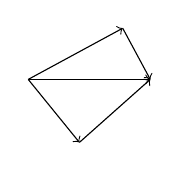
\begin{tikzpicture}
\draw[->] (0,0) -- (1.2,0.65);
\draw[->] (1.2,0.65) -- (1.55,0);
\draw[->] (0,0) -- (1.55,0);
\draw[->] (0,0) -- (0.65,-0.8);
\draw[->] (0.65,-0.8) -- (1.55,0);
\end{tikzpicture}
\end{center}
$\Lambda$ --- graph

$\Omega$ --- orientation

$M(\Lambda,\Omega)$ ---
[crossed out: \EnglishUnclear{GELFAND-P001444}{category-cancelled}{pr\ldots / cat\ldots [source beginnings]}]
the category of representations of the quiver.

$\mathcal D(\Lambda,\Omega)$ is the derived category of this category.

(1) \underline{Lemma.}

Then $\mathcal D(\Lambda,\Omega)$ does not depend on $\Omega$

($\mathcal D(\Lambda,\Omega_1)$ and $\mathcal D(\Lambda,\Omega_2)$ are equivalent)

for different $\Omega_1$ and $\Omega_2$.

\underline{Proof:} apply symmetry.

\underline{Problem:} find such
[crossed out: \EnglishUnclear{GELFAND-P001444}{derived-cancelled}{$\mathcal D^{\ell}(\mathcal A)$ / $\mathcal D^{e}(\mathcal A)$ / $\mathcal D^{b}(\mathcal A)$}]
subcategories $\mathcal A\subset\mathcal D(\Lambda,\Omega)$
that
\begin{equation*}
\mathcal D^{\ell}(\mathcal A)=\mathcal D(\Lambda,\Omega)
\end{equation*}
\EnglishUnclear{GELFAND-P001444}{subcategory-sign}{The sign between $\mathcal A$ and $\mathcal D(\Lambda,\Omega)$ is retraced: $\subset$; an angular sign $<$ / an earlier stroke is visible inside.}
\EnglishUnclear{GELFAND-P001444}{derived-exponent}{Upper index on $\mathcal D$: $\ell$ / $e$ / $b$.}

All of them have been found and are characterized by Dynkin graphs.

Reflections and gluings are used (and the ideas of perverse sheaves).

\underline{I.M.G.'s remark}
Vector bundles on $CP^n$ are classified only in the language of
derived categories.

\underline{Grothendieck:} through hard work, he obtained the concepts leading to the derived category
(like Michelangelo).

\underline{\underline{M.K.}}

\EnglishSourceFigure{GELFAND-P001444}{reflection-quiver}{On the left is a quiver with four vertices: $V_\alpha$ on the left, $V_\beta$ above, $V_\gamma$ on the right, and an unlabelled lower vertex. Arrows go from the left to the upper, right and lower vertices, and from the upper and lower vertices to the right. Above the edge $V_\alpha\to V_\beta$ is $f$; above the horizontal edge is a retraced or cancelled sign, uncertainly read as $g$ / $\varphi$. The label on this edge requires comparison with the original.}

\par\medskip\noindent
\begin{minipage}[c]{0.48\linewidth}\centering
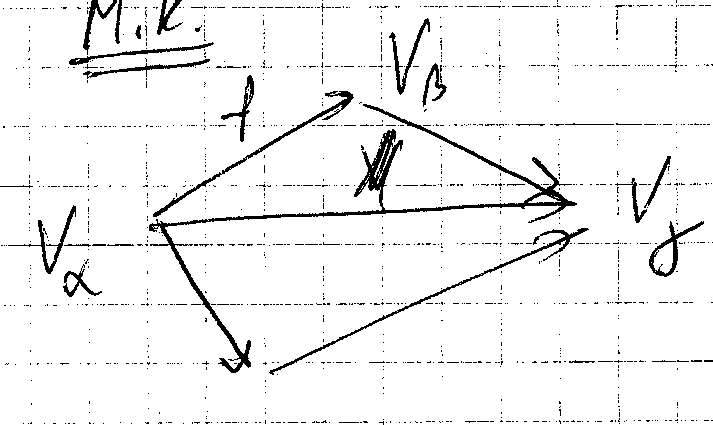
\includegraphics[width=\linewidth]{figures/gelfand-p001444-reflection-quiver-original.png}
\par\smallskip{\footnotesize Original manuscript diagram: GELFAND-P001444\par}
\end{minipage}\hfill
\begin{minipage}[c]{0.48\linewidth}\centering
\resizebox{\linewidth}{!}{% Partial recreation of five visible directed edges and readable vertex labels.
% The lower vertex is unlabelled in the source. The bracketed edge label is uncertain.
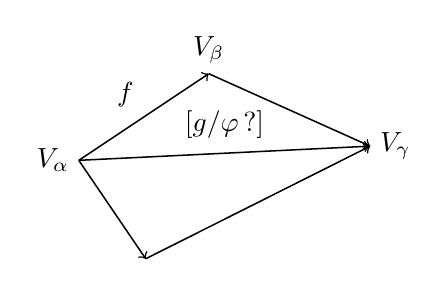
\begin{tikzpicture}[line width=0.55pt]
\coordinate (a) at (0,0);
\coordinate (b) at (1.65,1.10);
\coordinate (c) at (3.70,0.18);
\coordinate (d) at (0.85,-1.25);
\draw[->] (a)--node[above left]{$f$}(b);
\draw[->] (b)--(c);
\draw[->] (a)--(c);
\draw[->] (a)--(d);
\draw[->] (d)--(c);
\node[left] at (a) {$V_\alpha$};
\node[above] at (b) {$V_\beta$};
\node[right] at (c) {$V_\gamma$};
\node[above] at (1.85,0.15) {$[g/\varphi\,?]$};
\end{tikzpicture}
}
\par\smallskip{\footnotesize Partial recreation; the bracketed edge label gives unresolved candidates and may have been cancelled.\par}
\end{minipage}\par\medskip


\underline{Reflection} (a) $s_\alpha\Omega$ --- reverse the arrows
leaving $\alpha$.

(b)
\begin{equation*}
(s_\alpha V)_{\beta\ne\alpha}=V_\beta
\end{equation*}
\begin{equation*}
(s_\alpha V)_\alpha=\bigoplus_{\alpha\to\beta}V_\beta/(\text{the image of }V_\alpha)
\end{equation*}
with the corresponding maps.

There may be vectors in $V_\alpha$ which are sent to $0$ everywhere.

\begin{center}
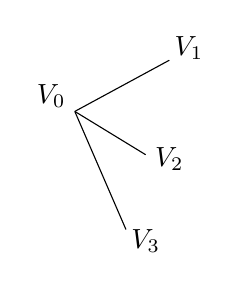
\begin{tikzpicture}
\node at (-0.3,0.2) {$V_0$};
\draw (0,0) -- (1.2,0.65);
\draw (0,0) -- (0.9,-0.55);
\draw (0,0) -- (0.65,-1.5);
\node at (1.45,0.8) {$V_1$};
\node at (1.2,-0.6) {$V_2$};
\node at (0.9,-1.65) {$V_3$};
\end{tikzpicture}
\end{center}
\begin{equation*}
V_0\longrightarrow V_1\oplus V_2\oplus V_3
\end{equation*}

